\documentclass[border=4pt]{standalone}
% Preámbulo común de las figuras. Cada figura es un documento standalone
% que se compila a SVG con scripts/build_figures.sh
\usepackage[utf8]{inputenc}
\usepackage{amsmath}
\usepackage{tikz}
\usepackage[american, siunitx]{circuitikz}
\usetikzlibrary{arrows.meta,calc,decorations.pathmorphing,patterns}
\tikzset{
  >={Stealth[length=2.2mm]},
  eje/.style={->, thin},
  hilo/.style={thick},
}
% Paleta común: tonos medios legibles sobre fondo claro
\definecolor{azul}{RGB}{31,94,168}
\definecolor{rojo}{RGB}{192,57,43}
\definecolor{verde}{RGB}{39,128,73}
\definecolor{naranja}{RGB}{211,120,30}
\definecolor{morado}{RGB}{125,60,152}

\begin{document}
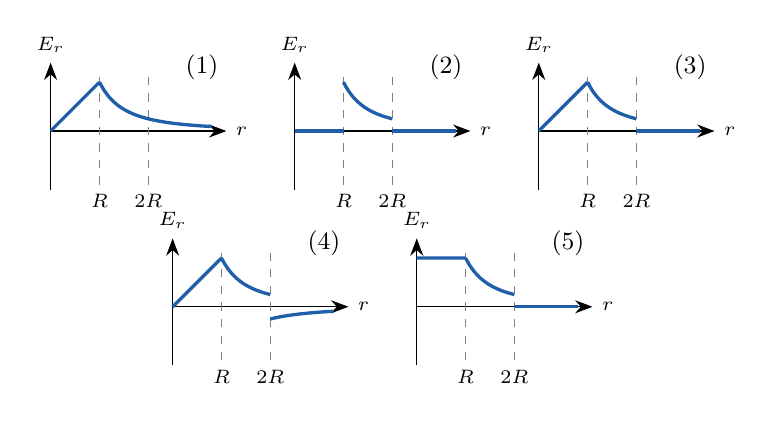
\begin{tikzpicture}[scale=0.62]
  \newcommand{\ejes}[2]{\begin{scope}[shift={#1}]
    \draw[->] (0,0) -- (3.6,0) node[right, font=\scriptsize]{$r$};
    \draw[->] (0,-1.2) -- (0,1.4) node[above, font=\scriptsize]{$E_r$};
    \draw[dashed, gray] (1,-1.1) -- (1,1.2) (2,-1.1) -- (2,1.2);
    \node[below, font=\scriptsize] at (1,-1.1) {$R$}; \node[below, font=\scriptsize] at (2,-1.1) {$2R$};
    \node[font=\small] at (3.1,1.3) {(#2)};
  \end{scope}}
  \ejes{(0,0)}{1} \ejes{(5,0)}{2} \ejes{(10,0)}{3} \ejes{(2.5,-3.6)}{4} \ejes{(7.5,-3.6)}{5}
  \begin{scope}[shift={(0,0)}] \draw[very thick, azul] (0,0) -- (1,1) plot[domain=1:3.3] (\x,{1/(\x*\x)}); \end{scope}
  \begin{scope}[shift={(5,0)}] \draw[very thick, azul] (0,0) -- (1,0); \draw[very thick, azul] plot[domain=1:2] (\x,{1/(\x*\x)}); \draw[very thick, azul] (2,0) -- (3.3,0); \end{scope}
  \begin{scope}[shift={(10,0)}] \draw[very thick, azul] (0,0) -- (1,1) plot[domain=1:2] (\x,{1/(\x*\x)}); \draw[very thick, azul] (2,0) -- (3.3,0); \end{scope}
  \begin{scope}[shift={(2.5,-3.6)}] \draw[very thick, azul] (0,0) -- (1,1) plot[domain=1:2] (\x,{1/(\x*\x)}); \draw[very thick, azul] plot[domain=2:3.3] (\x,{-1/(\x*\x)}); \end{scope}
  \begin{scope}[shift={(7.5,-3.6)}] \draw[very thick, azul] (0,1) -- (1,1) plot[domain=1:2] (\x,{1/(\x*\x)}); \draw[very thick, azul] (2,0) -- (3.3,0); \end{scope}
\end{tikzpicture}
\end{document}
